\documentclass[12pt, letterpaper]{article}
\usepackage[utf8]{inputenc}
\usepackage{graphicx}

\graphicspath{{./}}

\title{General refactor of "carstatus.cpp"}
\date{2019 November 15}
%\authors{Thomas De Min}

\begin{document}

\begin{titlepage}
\maketitle
\end{titlepage}

\begin{flushleft}

\section{Introduction}
	The SteeringWheel UI needs a lot of variables in order to works properly. In the past those variables were all putted toghether in one place, "carstatus". This class was created to store them and to collect methods associated to them. To date "carstatus" contains over 50 variables. At this point there is a lot of confusion and the code is difficult to be read.
\newline
\newline
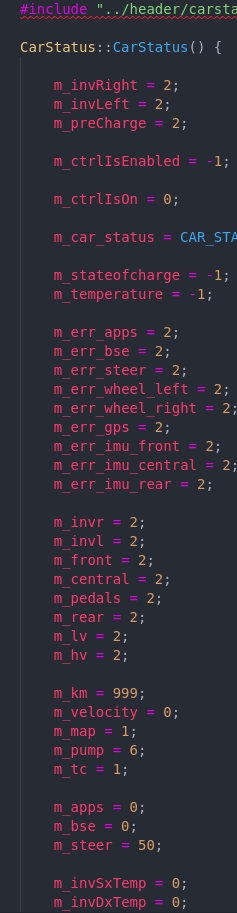
\includegraphics[scale=1.5]{code.png}
\newline
\newline
	The ideal solution is to store variables and methods associated in different classes and use them from "carstatus" using a "has a" for each class.\\
	---------------------------------------------INSERT CLASS DIAGRAM HERE-------------------------------------------------------

\section{Implementation issues}
	These changes will make code finally readable but some methods require to remain into "carstatus". These methods are thoose that deal with sendind changed data after emits.\\
	The only possible solution is to make some getters inside the new classes and call them from "carstatus.cpp". Therefore there will still be functions in this class but there will be much less.\\
	Another side effect of this implementation is the needs to create a ".h" (and ".cpp") file for each new class. There will be more or less 10 new classes, that means 10 new header files. So, in order to avoid too many duplications the refactor will limitate itself to implement only ".h" files and not ".cpp".

\section{Refactor}
\subsection{Inverter}
\begin{verbatim}
	int m_invRight;
	int m_invLeft;
	int m_preCharge;
	void setLeftInverterTemperature(int, int);
	void setRightInverterTemperature(int, int);
	QString HVStatus() const;
	void stopMessage(int);
	void setHVStatus(int, int, int)
\end{verbatim}

\end{flushleft}

\end{document}